\documentclass[conference]{IEEEtran}
\IEEEoverridecommandlockouts
% The preceding line is only needed to identify funding in the first footnote. If that is unneeded, please comment it out.
\usepackage{cite}
\usepackage{amsmath,amssymb,amsfonts}
\usepackage{algorithmic}
\usepackage{graphicx}
\usepackage{textcomp}
\usepackage{xcolor}
\def\BibTeX{{\rm B\kern-.05em{\sc i\kern-.025em b}\kern-.08em
    T\kern-.1667em\lower.7ex\hbox{E}\kern-.125emX}}
\begin{document}

\title{A Survey of Security Issues in Federated Laearning}

\author{\IEEEauthorblockN{1\textsuperscript{st} Yunhao Feng}
    \IEEEauthorblockA{\textit{National University of Defense and Technology} \\
        Changsha, China \\
        fengyunhaonudt@nudt.edu.cn}
    \and
    \IEEEauthorblockN{2\textsuperscript{nd} Yinjian Hou}
    \IEEEauthorblockA{\textit{National University of Defense and Technology} \\
        Changsha, China \\
        houyinjian18@nudt.edu.cn}

}

\maketitle

\begin{abstract}
    As people's awareness of the importance of personal privacy protection has grown,
    there has been a surge of interest in federated learning,
    which is a machine learning paradigm that enables training without requiring
    access to users' private data.
\end{abstract}



\section{Introduction}
The rapid development of digital technology has made the diversification, informationization,
and diversity of digital data the main topics of the current era. Meanwhile, deep learning (DL) has
demonstrated tremendous success in multiple fields, including computer vision, natural language
processing, and graphic networks. Clearly, using diverse data in deep learning models can effectively
improve their ability. However, there is also a growing interest in data privacy protection,
such as the General Data Protection Regulation (GDPR)\cite{b1}. On the other hand, data sources may
encounter the challenge of distributed storage, as is the case with data from mobile smart devices
or Internet of Things (IoT) scenarios\cite{b2},\cite{b3}. Therefore, utilizing these data to train models requires
overcoming limitations related to distribution and privacy\cite{b4}.

To solve these problems, federated learning(FL) is a machine learning paradigm proposed as a possible response to these
challenges\cite{b5}. FL enables collaborative model building among distributed members while ensuring sensitive data remains
within each participant's control\cite{b6}. Specifically, federated learning allows two or more participants to collaboratively
train a shared global DL model while keeping their training datasets locally. Each participant trains the shared model on its own
training data and exchanges and updates model parameters with other participants. Federated learning can improve the training speed
and the performance of the shared model while protecting privacy of the participants' training datasets\cite{b7}. Thus, it is a promising
technique for the scenarios where the training data is sensitive (e.g., medical records, personally identifiable information, etc.) \cite{b8},\cite{b9}.

\begin{figure}[htbp]
    \centerline{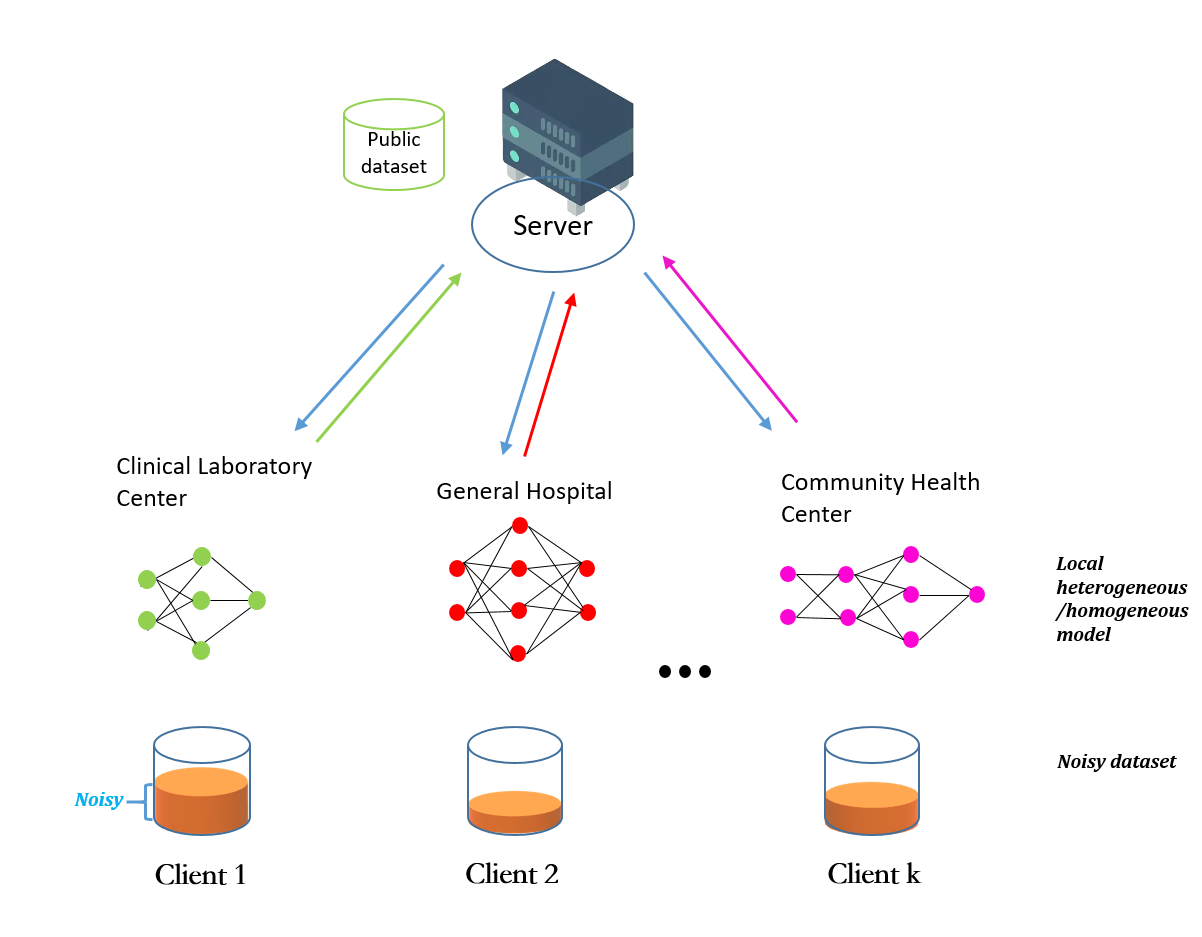
\includegraphics[width=0.8\linewidth,height=0.4\linewidth]{picture/f1.png}}
    \caption{A schematic of federated learning.}
    \label{fig1}
\end{figure}

Federated learning can be classified based on whether the participating datasets are the same, resulting in two types: homogeneous federated
learning  and heterogeneous federated learning \cite{b10},\cite{b11}. In homogeneous federated
learning, all participants have datasets with the same characteristics and data distribution, whereas in heterogeneous federated learning,
participants' datasets may differ in their characteristics and data distribution. The second classification of federated learning is based
on whether the models involved are the same, resulting in two types: horizontal federated learning and vertical
federated learning\cite{b12},\cite{b13}. In horizontal federated learning, all participants have the same model architecture, but may
have different local data\cite{b14}, while in vertical federated learning, each participant has a different model architecture but they collaborate on
processing the same set of data together\cite{b15}. The third way to classify federated learning is based on the type of task involved, resulting in several
types such as federated learning for clustering\cite{b16},\cite{b17}, federated learning for classification\cite{b18},\cite{b19}, federated learning for regression\cite{b20}, among others.
The fourth way to classify federated learning is based on the optimization approach used between the participants, resulting in several types such as
federated averaging\cite{b21},\cite{b22}, federated learning optimization, federated meta-learning\cite{b23}, and so on.

Federated learning methods currently face significant challenges related to their robustness, including backdoor attacks\cite{b24},\cite{b25},\cite{b26},\cite{b27},\cite{b28}, adversarial attacks\cite{b31},\cite{b32},\cite{b33},\cite{b34}, and Byzantine attacks\cite{b29},\cite{b30}. 
A backdoor attack involves a malicious participant in the federated learning process adding a backdoor to the model being trained, which can be triggered by a specific input pattern, 
allowing the attacker to control the output of the model in a targeted way. Adversarial attacks, on the other hand, entail adding small, 
carefully crafted perturbations to the input data to deceive the model and cause it to make incorrect predictions\cite{31},\cite{32}.   

\begin{figure}[htbp]
    \centerline{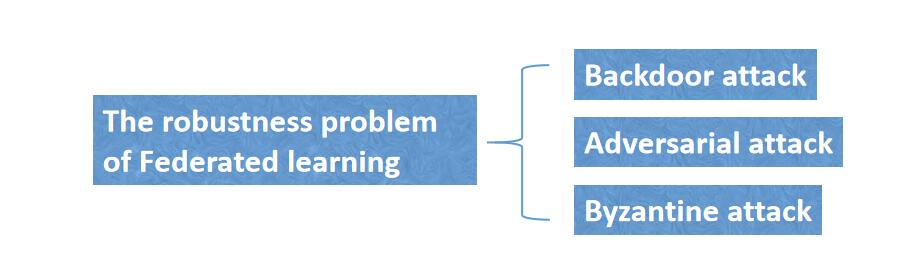
\includegraphics[width=0.8\linewidth,height=0.4\linewidth]{picture/f4.jpg}}
    \caption{The robust threat to federal learning}
    \label{fig2}
\end{figure}
And adversarial attacks can occur in federated learning when a malicious participant intentionally sends adversarial examples to the central server in an attempt to bias the model 
towards their own interests. This can be particularly problematic in applications such as personalized advertising or credit scoring, where the malicious participant may be motivated 
to gain an unfair advantage. Finally, Byzantine attacks involve one or more malicious participants in the federated learning process sending incorrect or misleading updates to the 
central server to disrupt the training process\cite{b35}.  

While federated learning can be vulnerable to certain types of attacks, there are techniques and approaches that can be used to improve the robustness and security of the process. 
It is important to carefully consider these issues when designing and implementing federated learning systems\cite{b38},\cite{b39}. 
For instance, knowledge distillation is a technique that can mitigate backdoor attacks by training a smaller\cite{b36}, 
distilled model using the output of the original model as the target labels. 
This can help remove any backdoor triggers that may have been added to the original model, as the smaller model won't be able to identify them. 
Another technique to mitigate backdoor attacks is model erasure\cite{b44}, where the model is trained to ignore specific input patterns that may be associated with the backdoor.  
\begin{figure}[htbp]
    \centerline{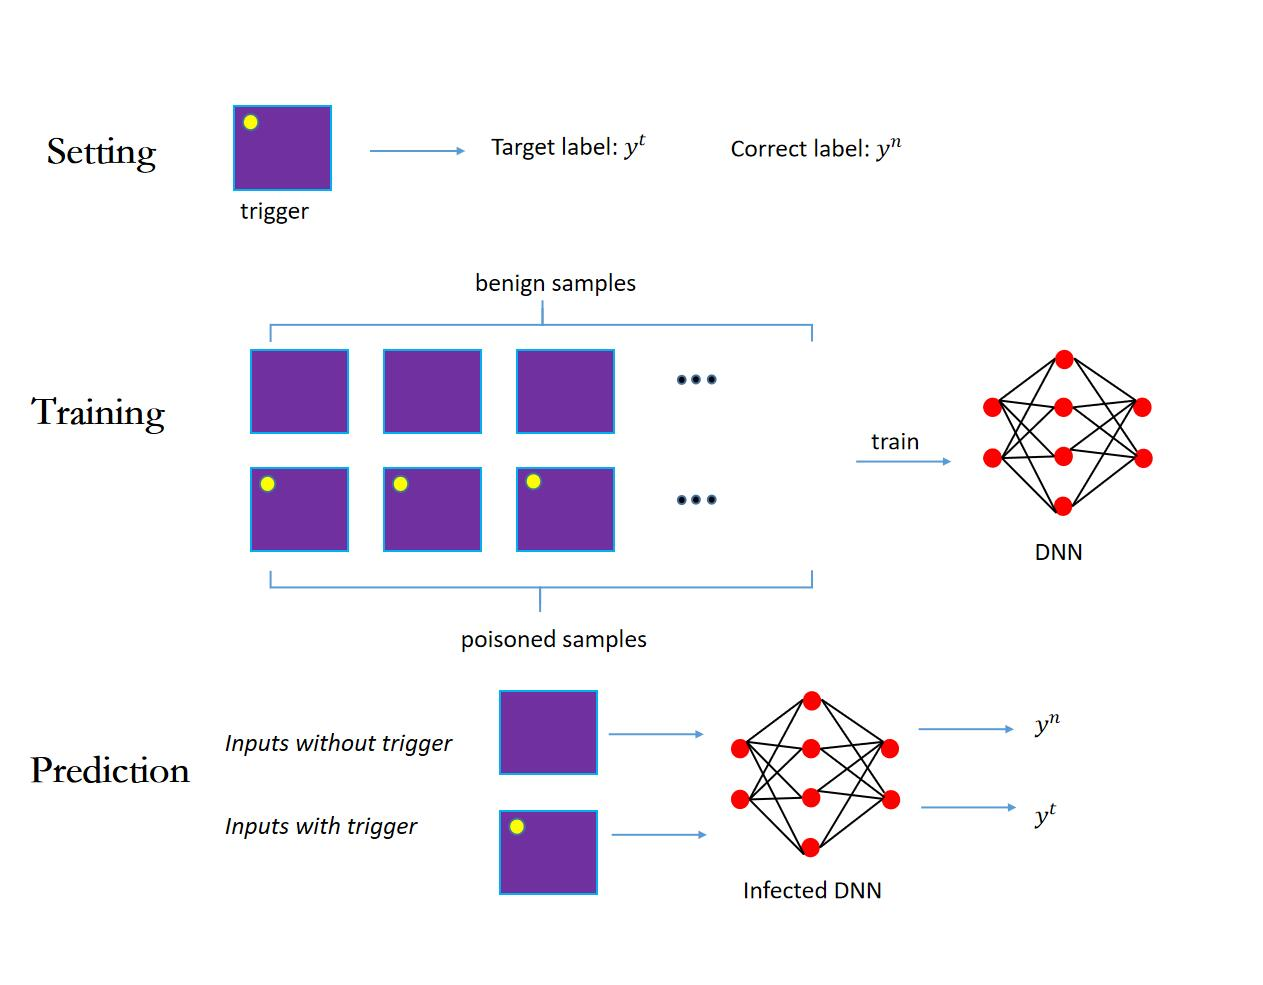
\includegraphics[width=0.8\linewidth,height=0.4\linewidth]{picture/f3.jpg}}
    \caption{Backdoor Attack}
    \label{fig3}
\end{figure}

Adversarial training is a technique that involves explicitly training the model to resist adversarial examples 
by adding adversarial perturbations to the training data\cite{b31},\cite{b32}.  
This can improve the model's ability to detect and resist adversarial attacks in federated learning settings.  
\begin{figure}[htbp]
    \centerline{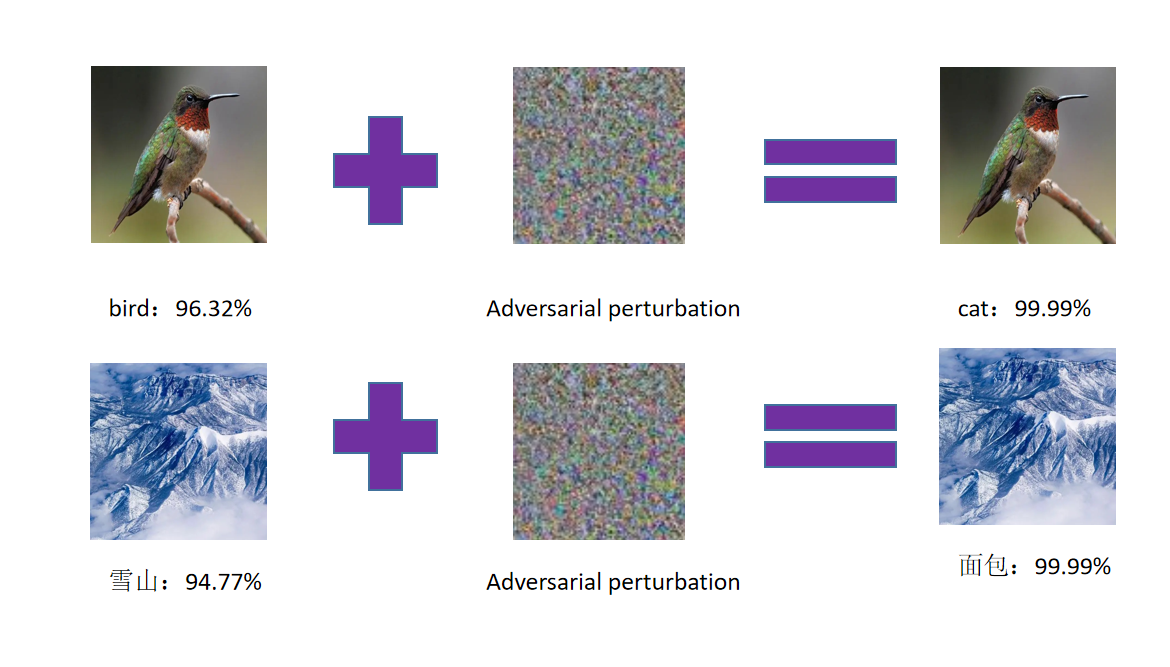
\includegraphics[width=0.8\linewidth,height=0.4\linewidth]{picture/f2.png}}
    \caption{Adversarial Attack}
    \label{fig4}
\end{figure}
Clustering can be used to identify malicious clients in federated learning systems subject to Byzantine attacks\cite{b35},\cite{b36}. 
The idea is to group participating clients based on the similarity of their updates, and to identify any clients whose updates are significantly different from the others. 
These clients can then be excluded from the training process, or their updates can be treated with greater suspicion to minimize the impact of their malicious behavior\cite{b37}.  
\begin{figure}[htbp]
    \centerline{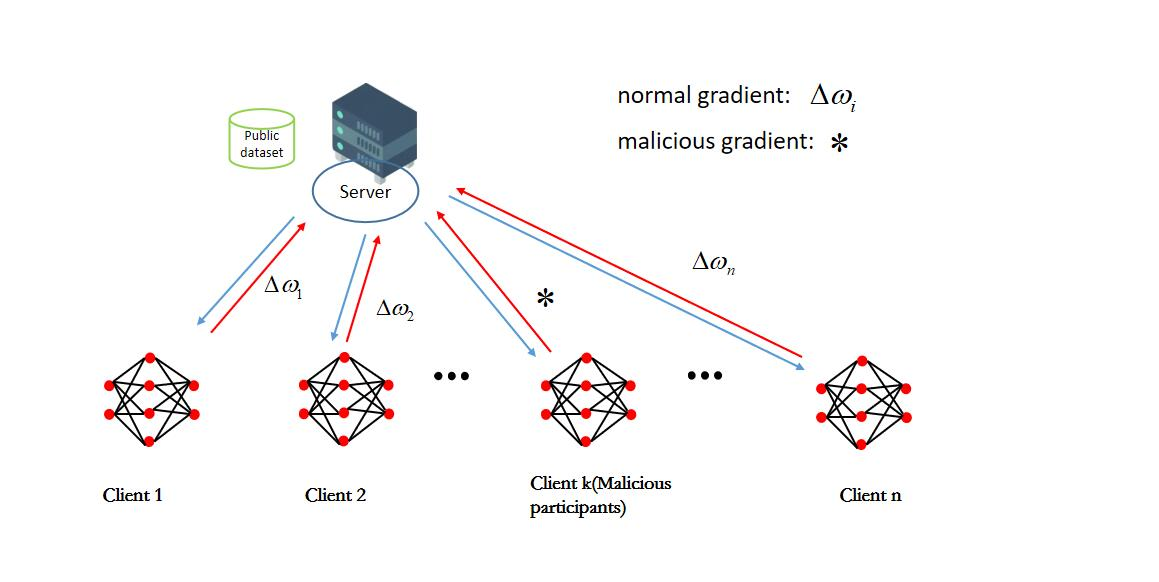
\includegraphics[width=0.8\linewidth,height=0.4\linewidth]{picture/f5.jpg}}
    \caption{Byzantine Attack}
    \label{fig5}
\end{figure}
This paper provides an overview of methods to increase the robustness of federated learning models, with the aim of enhancing the credibility and security of federated learning. 
While previous work has addressed the security of federated learning\cite{b39},\cite{b40},\cite{b41},\cite{b42},\cite{b43}, it has primarily focused on privacy leakage or backdoor attacks, 
with relatively few studies and reports on adversarial attacks. Building on prior work, this paper summarizes the attacks and defense methods of adversarial, backdoor, 
and Byzantine attacks in federated learning. A new classification method is proposed, supplementing the deficiencies of previous work on adversarial attacks. 
Moreover, this paper investigates a multi-level defense system against these attacks, and identifies open problems and future research directions for improving 
the robustness of federated learning.

\section{Ease of Use}

\subsection{Maintaining the Integrity of the Specifications}

The IEEEtran class file is used to format your paper and style the text. All margins,
column widths, line spaces, and text fonts are prescribed; please do not
alter them. You may note peculiarities. For example, the head margin
measures proportionately more than is customary. This measurement
and others are deliberate, using specifications that anticipate your paper
as one part of the entire proceedings, and not as an independent document.
Please do not revise any of the current designations.

\section{Prepare Your Paper Before Styling}
Before you begin to format your paper, first write and save the content as a
separate text file. Complete all content and organizational editing before
formatting. Please note sections \ref{AA}--\ref{SCM} below for more information on
proofreading, spelling and grammar.

Keep your text and graphic files separate until after the text has been
formatted and styled. Do not number text heads---{\LaTeX} will do that
for you.

\subsection{Abbreviations and Acronyms}\label{AA}
Define abbreviations and acronyms the first time they are used in the text,
even after they have been defined in the abstract. Abbreviations such as
IEEE, SI, MKS, CGS, ac, dc, and rms do not have to be defined. Do not use
abbreviations in the title or heads unless they are unavoidable.

\subsection{Units}
\begin{itemize}
    \item Use either SI (MKS) or CGS as primary units. (SI units are encouraged.) English units may be used as secondary units (in parentheses). An exception would be the use of English units as identifiers in trade, such as ``3.5-inch disk drive''.
    \item Avoid combining SI and CGS units, such as current in amperes and magnetic field in oersteds. This often leads to confusion because equations do not balance dimensionally. If you must use mixed units, clearly state the units for each quantity that you use in an equation.
    \item Do not mix complete spellings and abbreviations of units: ``Wb/m\textsuperscript{2}'' or ``webers per square meter'', not ``webers/m\textsuperscript{2}''. Spell out units when they appear in text: ``. . . a few henries'', not ``. . . a few H''.
    \item Use a zero before decimal points: ``0.25'', not ``.25''. Use ``cm\textsuperscript{3}'', not ``cc''.)
\end{itemize}

\subsection{Equations}
Number equations consecutively. To make your
equations more compact, you may use the solidus (~/~), the exp function, or
appropriate exponents. Italicize Roman symbols for quantities and variables,
but not Greek symbols. Use a long dash rather than a hyphen for a minus
sign. Punctuate equations with commas or periods when they are part of a
sentence, as in:
\begin{equation}
    a+b=\gamma\label{eq}
\end{equation}

Be sure that the
symbols in your equation have been defined before or immediately following
the equation. Use ``\eqref{eq}'', not ``Eq.~\eqref{eq}'' or ``equation \eqref{eq}'', except at
the beginning of a sentence: ``Equation \eqref{eq} is . . .''

\subsection{\LaTeX-Specific Advice}

Please use ``soft'' (e.g., \verb|\eqref{Eq}|) cross references instead
of ``hard'' references (e.g., \verb|(1)|). That will make it possible
to combine sections, add equations, or change the order of figures or
citations without having to go through the file line by line.

Please don't use the \verb|{eqnarray}| equation environment. Use
\verb|{align}| or \verb|{IEEEeqnarray}| instead. The \verb|{eqnarray}|
environment leaves unsightly spaces around relation symbols.

Please note that the \verb|{subequations}| environment in {\LaTeX}
will increment the main equation counter even when there are no
equation numbers displayed. If you forget that, you might write an
article in which the equation numbers skip from (17) to (20), causing
the copy editors to wonder if you've discovered a new method of
counting.

    {\BibTeX} does not work by magic. It doesn't get the bibliographic
data from thin air but from .bib files. If you use {\BibTeX} to produce a
bibliography you must send the .bib files.

    {\LaTeX} can't read your mind. If you assign the same label to a
subsubsection and a table, you might find that Table I has been cross
referenced as Table IV-B3.

{\LaTeX} does not have precognitive abilities. If you put a
\verb|\label| command before the command that updates the counter it's
supposed to be using, the label will pick up the last counter to be
cross referenced instead. In particular, a \verb|\label| command
should not go before the caption of a figure or a table.

Do not use \verb|\nonumber| inside the \verb|{array}| environment. It
will not stop equation numbers inside \verb|{array}| (there won't be
any anyway) and it might stop a wanted equation number in the
surrounding equation.

\subsection{Some Common Mistakes}\label{SCM}
\begin{itemize}
    \item The word ``data'' is plural, not singular.
    \item The subscript for the permeability of vacuum $\mu_{0}$, and other common scientific constants, is zero with subscript formatting, not a lowercase letter ``o''.
    \item In American English, commas, semicolons, periods, question and exclamation marks are located within quotation marks only when a complete thought or name is cited, such as a title or full quotation. When quotation marks are used, instead of a bold or italic typeface, to highlight a word or phrase, punctuation should appear outside of the quotation marks. A parenthetical phrase or statement at the end of a sentence is punctuated outside of the closing parenthesis (like this). (A parenthetical sentence is punctuated within the parentheses.)
    \item A graph within a graph is an ``inset'', not an ``insert''. The word alternatively is preferred to the word ``alternately'' (unless you really mean something that alternates).
    \item Do not use the word ``essentially'' to mean ``approximately'' or ``effectively''.
    \item In your paper title, if the words ``that uses'' can accurately replace the word ``using'', capitalize the ``u''; if not, keep using lower-cased.
    \item Be aware of the different meanings of the homophones ``affect'' and ``effect'', ``complement'' and ``compliment'', ``discreet'' and ``discrete'', ``principal'' and ``principle''.
    \item Do not confuse ``imply'' and ``infer''.
    \item The prefix ``non'' is not a word; it should be joined to the word it modifies, usually without a hyphen.
    \item There is no period after the ``et'' in the Latin abbreviation ``et al.''.
    \item The abbreviation ``i.e.'' means ``that is'', and the abbreviation ``e.g.'' means ``for example''.
\end{itemize}
An excellent style manual for science writers is \cite{b7}.

\subsection{Authors and Affiliations}
\textbf{The class file is designed for, but not limited to, six authors.} A
minimum of one author is required for all conference articles. Author names
should be listed starting from left to right and then moving down to the
next line. This is the author sequence that will be used in future citations
and by indexing services. Names should not be listed in columns nor group by
affiliation. Please keep your affiliations as succinct as possible (for
example, do not differentiate among departments of the same organization).

\subsection{Identify the Headings}
Headings, or heads, are organizational devices that guide the reader through
your paper. There are two types: component heads and text heads.

Component heads identify the different components of your paper and are not
topically subordinate to each other. Examples include Acknowledgments and
References and, for these, the correct style to use is ``Heading 5''. Use
``figure caption'' for your Figure captions, and ``table head'' for your
table title. Run-in heads, such as ``Abstract'', will require you to apply a
style (in this case, italic) in addition to the style provided by the drop
down menu to differentiate the head from the text.

Text heads organize the topics on a relational, hierarchical basis. For
example, the paper title is the primary text head because all subsequent
material relates and elaborates on this one topic. If there are two or more
sub-topics, the next level head (uppercase Roman numerals) should be used
and, conversely, if there are not at least two sub-topics, then no subheads
should be introduced.

\subsection{Figures and Tables}
\paragraph{Positioning Figures and Tables} Place figures and tables at the top and
bottom of columns. Avoid placing them in the middle of columns. Large
figures and tables may span across both columns. Figure captions should be
below the figures; table heads should appear above the tables. Insert
figures and tables after they are cited in the text. Use the abbreviation
``Fig.~\ref{fig}'', even at the beginning of a sentence.

\begin{table}[htbp]
    \caption{Table Type Styles}
    \begin{center}
        \begin{tabular}{|c|c|c|c|}
            \hline
            \textbf{Table} & \multicolumn{3}{|c|}{\textbf{Table Column Head}}                                                         \\
            \cline{2-4}
            \textbf{Head}  & \textbf{\textit{Table column subhead}}           & \textbf{\textit{Subhead}} & \textbf{\textit{Subhead}} \\
            \hline
            copy           & More table copy$^{\mathrm{a}}$                   &                           &                           \\
            \hline
            \multicolumn{4}{l}{$^{\mathrm{a}}$Sample of a Table footnote.}
        \end{tabular}
        \label{tab1}
    \end{center}
\end{table}

\begin{figure}[htbp]
    \centerline{
\includegraphics{fig1.png}}
    \caption{Example of a figure caption.}
    \label{fig}
\end{figure}

Figure Labels: Use 8 point Times New Roman for Figure labels. Use words
rather than symbols or abbreviations when writing Figure axis labels to
avoid confusing the reader. As an example, write the quantity
``Magnetization'', or ``Magnetization, M'', not just ``M''. If including
units in the label, present them within parentheses. Do not label axes only
with units. In the example, write ``Magnetization (A/m)'' or ``Magnetization
\{A[m(1)]\}'', not just ``A/m''. Do not label axes with a ratio of
quantities and units. For example, write ``Temperature (K)'', not
``Temperature/K''.

\section*{Acknowledgment}

The preferred spelling of the word ``acknowledgment'' in America is without
an ``e'' after the ``g''. Avoid the stilted expression ``one of us (R. B.
G.) thanks $\ldots$''. Instead, try ``R. B. G. thanks$\ldots$''. Put sponsor
acknowledgments in the unnumbered footnote on the first page.



\begin{thebibliography}{00}
    \bibitem{b1} M. Goddard, The EU General Data Protection Regulation (GDPR): European regulation that has a global impact, International Journal of Market Research 59 (2017) 703–705.
    \bibitem{b2} O. Gómez-Carmona, D. Casado-Mansilla, F. A. Kraemer, D. L. de Ipiña, J. GarcíaZubia, Exploring the computational cost of machine learning at the edge for human-centric internet of things, Future Generation Computer Systems 112 (2020) 670–683.
    \bibitem{b3} J. Zhang, D. Tao, Empowering things with intelligence: A survey of the progress, challenges, and opportunities in artificial intelligence of things, IEEE Internet of Things Journal 8 (2021) 7789–7817.
    \bibitem{b4} C. Ma, J. Koneˇcný, M. Jaggi, V. Smith, M. Jordan, P. Richtárik, M. Takáˇc, Distributed optimization with arbitrary local solvers, Optimization Methods and Software 32 (2017) 813–848.
    \bibitem{b5} Brendan McMahan, Eider Moore, Daniel Ramage, Seth Hampson, and Blaise Aguera y Arcas. Communication-Efficient Learning of Deep Networks from Decentralized Data. In Proceedings of the 20th International Conference on Artificial Intelligence and Statistics, volume 54 of Proceedings of Machine Learning Research, pages 1273–1282. PMLR, 20–22 Apr 2017.
    \bibitem{b6} GlobalFederatedLearningMarketbyApplication (Drug Discovery, Industrial IoT, Risk Management), Vertical (Healthcare  Life Sciences, BFSI, Manufacturing, Automotive Transportation, Energy  Utilities), and Region - Forecast to 2028, "researchandmarkets.com", Accessed date: May 12, 2023.
    \bibitem{b7} Q. Yang, Y. Liu, Y. Cheng, Y. Kang, T. Chen, H. Yu, Federated Learning, Synthesis Lectures on Artificial Intelligence and Machine Learning, 2019.
    \bibitem{b8} M. Househ, E. Borycki, and A. Kushniruk. Multiple Perspectives on Artificial Intelligence in Healthcare. Springer, 2021.
    \bibitem{b9} R. Rau, R. Wardrop, and L. Zingales. The Palgrave Handbook of Technological Finance. Springer, 2021.
    \bibitem{b10} Fang, Xiuwen, and Mang Ye. "Robust federated learning with noisy and heterogeneous clients." Proceedings of the IEEE/CVF Conference on Computer Vision and Pattern Recognition. 2022.
    \bibitem{b11} Tang, Zhenheng, et al. "Virtual homogeneity learning: Defending against data heterogeneity in federated learning." International Conference on Machine Learning. PMLR, 2022.
    \bibitem{b12} Kairouz, Peter, et al. "Advances and open problems in federated learning." Foundations and Trends® in Machine Learning 14.1–2 (2021): 1-210.
    \bibitem{b13} Yang, Qiang, et al. "Federated machine learning: Concept and applications." ACM Transactions on Intelligent Systems and Technology (TIST) 10.2 (2019): 1-19.
    \bibitem{b14} Huang, Wei, et al. "Fairness and accuracy in horizontal federated learning." Information Sciences 589 (2022): 170-185.
    \bibitem{b15} Liu, Yang, et al. "Vertical federated learning." arXiv preprint arXiv:2211.12814 (2022).
    \bibitem{b16} Ghosh, Avishek, et al. "An efficient framework for clustered federated learning." Advances in Neural Information Processing Systems 33 (2020): 19586-19597.
    \bibitem{b17} Briggs, Christopher, Zhong Fan, and Peter Andras. "Federated learning with hierarchical clustering of local updates to improve training on non-IID data." 2020 International Joint Conference on Neural Networks (IJCNN). IEEE, 2020.
    \bibitem{b18} Hsu, Tzu-Ming Harry, Hang Qi, and Matthew Brown. "Federated visual classification with real-world data distribution." Computer Vision–ECCV 2020: 16th European Conference, Glasgow, UK, August 23–28, 2020, Proceedings, Part X 16. Springer International Publishing, 2020.
    \bibitem{b19} Wahab, Omar Abdel, et al. "Federated machine learning: Survey, multi-level classification, desirable criteria and future directions in communication and networking systems." IEEE Communications Surveys and Tutorials 23.2 (2021): 1342-1397.
    \bibitem{b20} Yang, Shengwen, et al. "Parallel distributed logistic regression for vertical federated learning without third-party coordinator." arXiv preprint arXiv:1911.09824 (2019).
    \bibitem{b21} Deng, Yuyang, Mohammad Mahdi Kamani, and Mehrdad Mahdavi. "Distributionally robust federated averaging." Advances in neural information processing systems 33 (2020): 15111-15122.
    \bibitem{b22} Sun, Tao, Dongsheng Li, and Bao Wang. "Decentralized federated averaging." IEEE Transactions on Pattern Analysis and Machine Intelligence 45.4 (2022): 4289-4301.
    \bibitem{b23} Fallah, Alireza, Aryan Mokhtari, and Asuman Ozdaglar. "Personalized federated learning: A meta-learning approach." arXiv preprint arXiv:2002.07948 (2020).  
    \bibitem{b24} Bagdasaryan, Eugene, et al. "How to backdoor federated learning." International conference on artificial intelligence and statistics. PMLR, 2020.  
    \bibitem{b25} Wang, Hongyi, et al. "Attack of the tails: Yes, you really can backdoor federated learning." Advances in Neural Information Processing Systems 33 (2020): 16070-16084.   
    \bibitem{b26} Gong, Xueluan, et al. "Backdoor attacks and defenses in federated learning: State-of-the-art, taxonomy, and future directions." IEEE Wireless Communications (2022).  
    \bibitem{b27} Sun, Ziteng, et al. "Can you really backdoor federated learning?." arXiv preprint arXiv:1911.07963 (2019).  
    \bibitem{b28} Ozdayi, Mustafa Safa, Murat Kantarcioglu, and Yulia R. Gel. "Defending against backdoors in federated learning with robust learning rate." Proceedings of the AAAI Conference on Artificial Intelligence. Vol. 35. No. 10. 2021.  
    \bibitem{b29} Fang, Minghong, et al. "Local model poisoning attacks to {Byzantine-Robust} federated learning." 29th USENIX security symposium (USENIX Security 20). 2020.  
    \bibitem{b30} Guo, Shangwei, et al. Byzantine-Resilient Decentralized Stochastic Gradient Descent.  
    \bibitem{b31} Zizzo, Giulio, et al. "Fat: Federated adversarial training." arXiv preprint arXiv:2012.01791 (2020).  
    \bibitem{b32} Chen, Chen, et al. "Calfat: Calibrated federated adversarial training with label skewness." Advances in Neural Information Processing Systems 35 (2022): 3569-3581.  
    \bibitem{b33} Li, Xiaoxiao, Zhao Song, and Jiaming Yang. "Federated adversarial learning: A framework with convergence analysis." International Conference on Machine Learning. PMLR, 2023.  
    \bibitem{b34} Zhang, Jie, et al. "Delving into the adversarial robustness of federated learning." arXiv preprint arXiv:2302.09479 (2023).  
    \bibitem{b35} Prakash, Saurav, and Amir Salman Avestimehr. "Mitigating byzantine attacks in federated learning." arXiv preprint arXiv:2010.07541 (2020).   
    \bibitem{b36} Huang, Hanxun, et al. "Distilling Cognitive Backdoor Patterns within an Image." arXiv preprint arXiv:2301.10908 (2023).   
    \bibitem{b37} Blanchard, Peva, et al. "Machine learning with adversaries: Byzantine tolerant gradient descent." Advances in neural information processing systems 30 (2017).   
    \bibitem{b38} Lyu, Lingjuan, et al. "Privacy and robustness in federated learning: Attacks and defenses." IEEE transactions on neural networks and learning systems (2022).    
    \bibitem{b39} Guo, Shangwei, et al. "Robust and privacy-preserving collaborative learning: A comprehensive survey." arXiv preprint arXiv:2112.10183 (2021).    
    \bibitem{b40} Enthoven, David, and Zaid Al-Ars. "An overview of federated deep learning privacy attacks and defensive strategies." Federated Learning Systems: Towards Next-Generation AI (2021): 173-196.  
    \bibitem{b41} Rodríguez-Barroso, Nuria, et al. "Survey on federated learning threats: Concepts, taxonomy on attacks and defences, experimental study and challenges." Information Fusion 90 (2023): 148-173.  
    \bibitem{b42} Tariq, Asadullah, et al. "Trustworthy Federated Learning: A Survey." arXiv preprint arXiv:2305.11537 (2023).   
    \bibitem{b43} Zhang, Yifei, et al. "A Survey of Trustworthy Federated Learning with Perspectives on Security, Robustness, and Privacy." arXiv preprint arXiv:2302.10637 (2023).  
    \bibitem{b44} Dal Fabbro, Nicolò, Aritra Mitra, and George J. Pappas. "Federated TD Learning over Finite-Rate Erasure Channels: Linear Speedup under Markovian Sampling." IEEE Control Systems Letters (2023).  










\end{thebibliography}


\end{document}
